\documentclass[a4paper, 10pt, final, garamond]{book}
\usepackage{cours-preambule}

\makeatletter
\renewcommand{\@chapapp}{Devoir surveill\'e -- num\'ero}
\makeatother

\begin{document}
\setcounter{chapter}{2}

\def\lspace{25}

\chapter{Commentaires sur le DS \oldno3}

\section{Commentaires généraux}
\subsection{Appréciation globale}

C'est un DS qui a vu de grandes réussites, mais en moyenne le niveau ne décolle
pas. Il est probable que ce DS soit le plus facile de cette année. Les
connaissances interrogées sont manipulées depuis plus d'un mois et les méthodes
utilisées sont répétitives. Malheureusement, l'écart se creuse et les techniques
fondamentales sont loin d'être maîtrisées pour un majorité de la classe.

Le premier exercice était une répétition du cours et des interrogations, collant
presque trait pour trait à l'exercice TDTM2\_ent|I/. Il en était de même pour le
deuxième exercice~: on avait vu une situation pratiquement en tous points
similaires dans l'exercice TDTM2\_app|III/, avec quelques questions qui
demandaient un peu plus d'analyse de votre part. À la limite, cela se comprend,
on a moins pratiqué la transformation de la matière.

\noindent
\begin{isd}[righthand ratio=.7]
	En revanche, à partir de l'exercice 3, le manque de maîtrise, est fâcheux.
	Pour preuve, la moyenne de cet exercice~: moins de la moitié des points pour
	un exercice pratiquement copié-collé du cours, c'est anormal. Il y a bien
	quelques connaissances présentes chez tout le monde et les efforts fournis par
	l'ensemble de la classe sont certains, mais les méthodes vues, revues et
	répétées sont difficile à ancrer.

	De même pour le problème 1, qui est une amélioration mais sinon un copié-collé
	de l'exercice TDE4-E5\_ent|II/, fait intégralement en TD à la rentrée, avec
	une détermination des conditions initiales en plus. Vous ne vous êtes pas
	approprié les TDs et les conseils donnés en classe. Beaucoup de schémas
	équivalents ont été fait, mais l'analyse des régimes permanents et
	l'utilisation des dipôles équivalents sont encore lacunaires.

	Curieusement, le problème 2 reste mieux réussi, sans pour autant avoir
	commencé la mécanique. L'établissement du système est encore mal faite et le
	nombre de problèmes de vecteurs et de projections est toujours grand, mais
	dans l'ensemble il vous a rapporté pas mal de points.
	\tcblower
	\begin{center}
		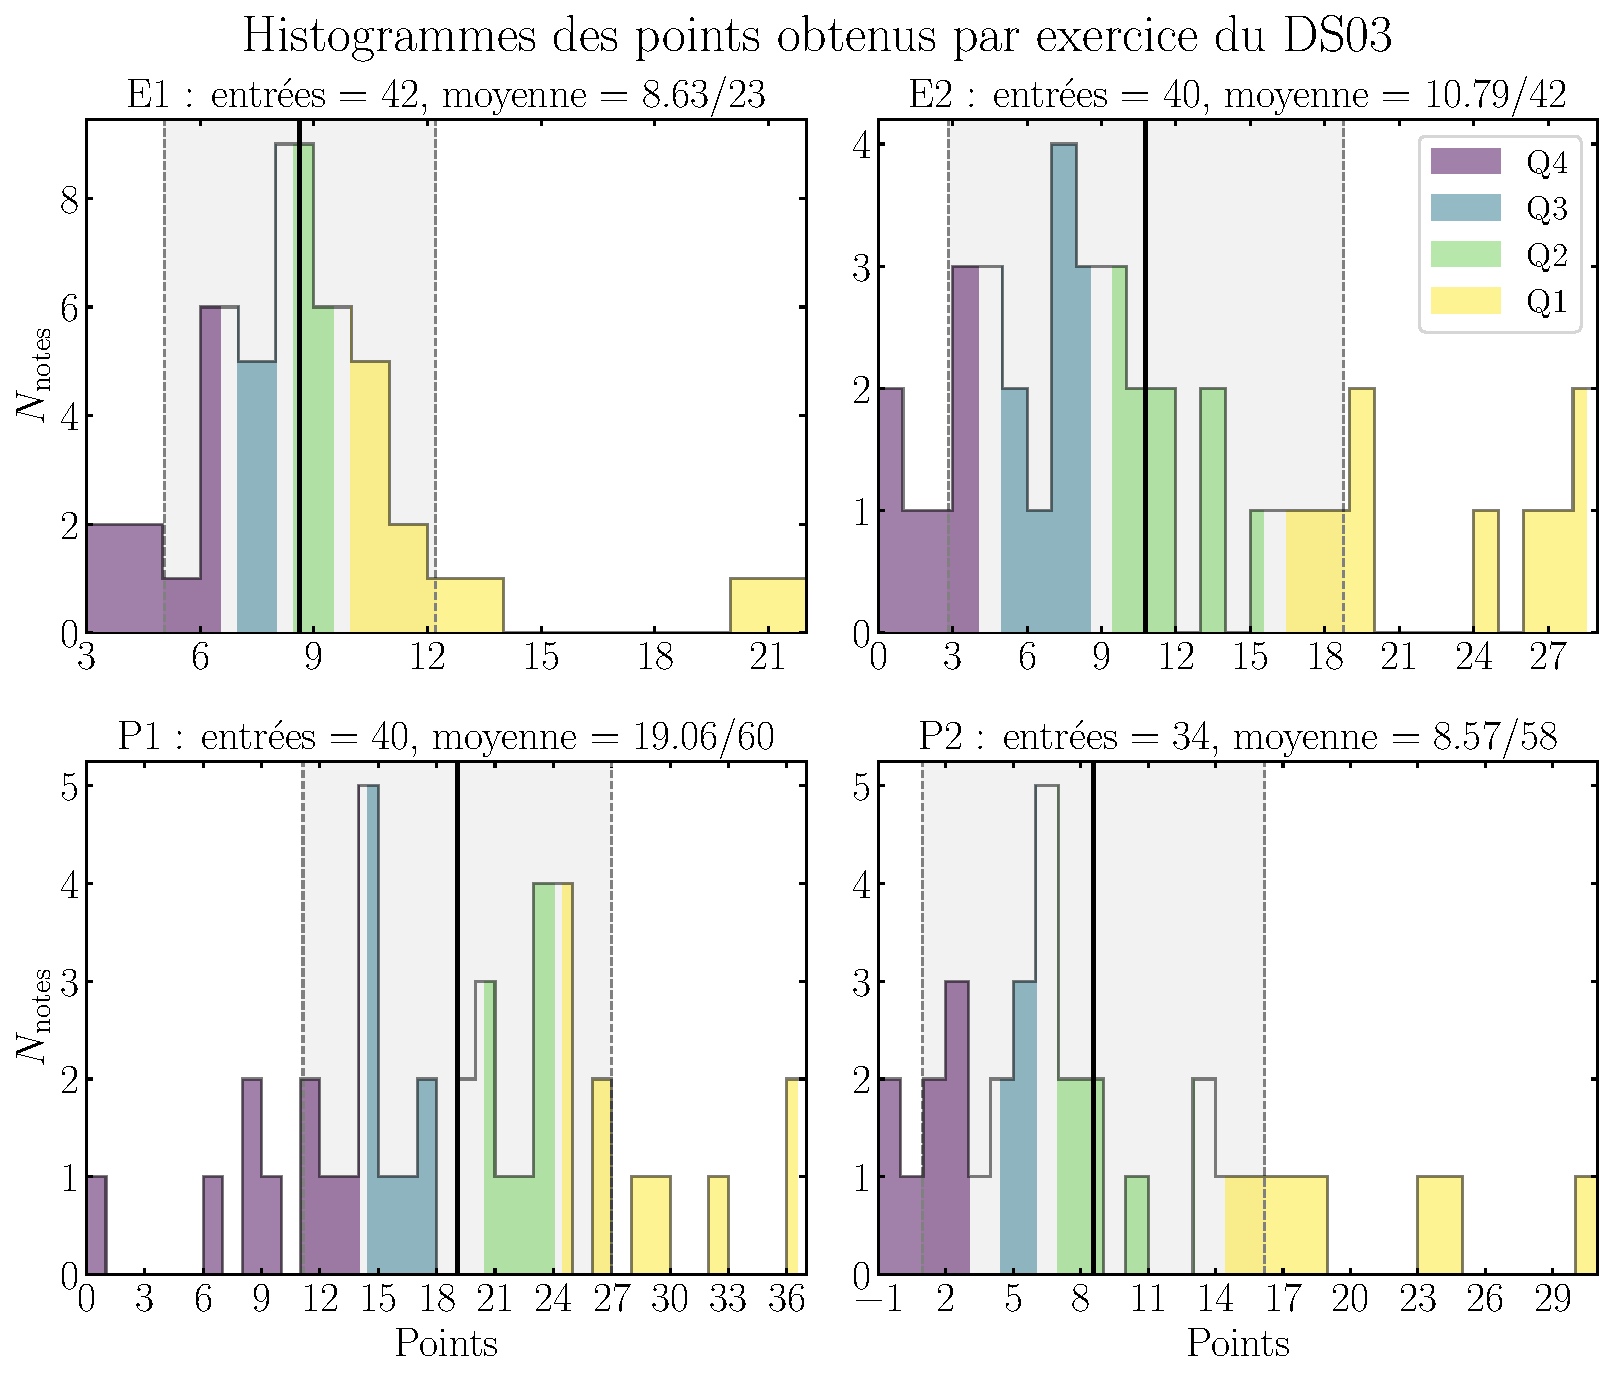
\includegraphics[width=\linewidth]{DS03_hist_all.pdf}
	\end{center}
\end{isd}

\subsection{Sur la forme}
\begin{tcn}[cnt, bld](impo)<lftt>{Attention}
	\large Faites attention à rendre vos copies doubles dans le bon sens~!!
\end{tcn}
C'est parfois un puzzle pour retrouver l'ordre des problèmes et questions, j'ai
mieux à faire de mon temps que de comprendre dans quel sens il faut tourner 2 ou
3 copies doubles. Malus $-$Q.
\begin{tcn}(inte)<lftt>{Astuce}
	Dès que vous changez de copie, mettez votre nom, prénom en haut à gauche, et
	le numéro de copie en bas à droite~: vous saurez quelle est la première page
	de la copie et ça sera même plus facile pour vous y repérer vous-même.
\end{tcn}

\subsection{Commentaires principaux et récurrents}

Il reste des incompréhensions \textbf{profondes}.
\begin{tcn}(prop)"bomb"{Attention}
	\vspace{-15pt}
	\begin{gather*}
		C\dv{u}{t}
		\quad
		\text{n'est pas le produit des nombres $C$, $u$ et $d$ sur $d \cdot t$~!! On
			ne peut pas l'écrire}
		\quad
		\dcancel{u \dv{C}{t}}
		\quad
		\text{\faIcon{skull-crossbones}}
		% \text{\faTimes}
		\\
		\beforetext{C'est}
		Q_{r} = \frac{\boxed{\prod_{i}} a(\ce{P_i})^{\nu_i}}{\prod_{i}
			a(\ce{R_i})^{\nu_i}}
		\qMath{et pas}
		Q_{r} = \frac{\dcancel{\sum_{i}} a(\ce{P_i})^{\nu_i}}{\prod_{i}
			a(\ce{R_i})^{\nu_i}}
		\\
		\beforetext{C'est}
		a (\ce{X}\ind{état})
		\qMath{et pas}
		a \left(\frac{P_{\ce{X}}}{p^\circ}\right)
		\qou
		a (\ce{X})\ind{état}
	\end{gather*}
\end{tcn}
Très peu de «~on insère la forme générique $u(t) = K \exr^{rt}$~». Je ne les
avais pas inclus dans les corrigés de l'année dernière, mais ça reste
important~!
\smallbreak
Nombre d'entre vous a oublié de dériver les produits de fonctions pour la
seconde condition initiale… c'est dommage.

\setcounter{section}{0}
\section[30]"E"{Synthèse de l'ammoniac}
\begin{enumerate}
	\item[n]{5} % Q1
	      Bien. Il faut \textbf{remplacer} $n_{\ce{H_2}}$ par son expression en
	      fonction de $n_0$. Attention à la colonne $n\ind{tot, gaz}$.
	      \smallbreak
	      Ne vous trompez pas bêtement sur les proportions stœchiométriques~! Ça
	      n'est pas pour rien qu'on vous apprend à tout démonrer à partir de
	      définitions simples… si vous n'êtes pas sûr-es, vérifier que les deux
	      quantités de matière que vous avez écrites s'annulent en même temps
	      pour $\xi\ind{max}$~!
	\item[n]{4} % Q2
	      Ne pas confondre équilibre et maximal~! C'est $\xi\ind{max}$ qui vaut
	      $n_0$.
	      \smallbreak
	      \textbf{Ça n'est pas parce qu'on est dans les proportions
		      stœchiométriques que l'avancement est maximal}~!!
	\item[n]{7} % Q3
	      \faIcon{exclamation-triangle} J'ai combiné les questions 3 et 4 pour
	      condenser le corrigé.
	      \smallbreak
	      \textbf{Simplifiez les fractions de fractions} ($P_{\ce{X}}/P^\circ$ ou
	      $n_{\ce{X}}/n\ind{tot}$) dans l'expression de $K^\circ$~!
	      \smallbreak
	      Explicitez l'expression des activités des constituants.
	\item[n]{2} % Q4
	      \textbf{Il faut vraiment distinguer vos lettres}~:
	      \begin{center}
		      \Large $\rho \neq p$
	      \end{center}
	\item[n]{10} % Q5
	      Une pincée de bonnes réponses. \textbf{Ayez le réflexe de prendre la
		      racine carrée} de $K^\circ$ dans les situations où on obtiendrait un
	      polynôme de degré supérieur strict à 2.
	\item[n]{3} % Q6
	      Attention à ne pas confondre $Q_r$ avec $K^\circ$~! Si on diminue la
	      pression, on \textbf{augmente $\boxed{Q_r}$}~; $K^\circ$ c'est une
	      constante (enfin, dépend de la température). Donc on amène va de
	      $Q_{r,\eql} = K^\circ$ à $Q_{r} > K^\circ$~: sens indirect.
\end{enumerate}

\section[38]"E"{Réaction du dibromure de cuivre}
\begin{enumerate}
	\item[n]{4} % Q1
	      Toujours écrire la loi d'action de masse. \textbf{Attention à l'unité de
		      $p^\circ$}~: $\boxed{p^\circ = \SI{1}{bar}}$, donc ici $K^\circ =
		      \num{52.6e-3}$~! Ne convertissez pas quelque chose sans unité en une
	      autre unité…
	      \smallbreak
	      Ne confondez pas un produit ($\cdot $) avec une somme~!! Aïe.
	      \smallbreak
	      \textbf{Il faut savoir convertir les celsius en kelvins}~!!!
	\item[n]{13} % Q2
	      Différenciez bien $P\ind{eq}$, $P_f$, précisez de quelle quantité de
	      matière
	      vous parlez… Mentionner la \textbf{rupture d'équilibre}.
	      \smallbreak
	      Composition à l'état final $\Ra $ composition de \textbf{tous les
		      constituants}~! Pas que $\ce{Br_2_{\gaz}}$…
	      \smallbreak
	      $n\ind{tot,gaz}$ ne prend en compte que les gaz, pas les solides~!
	      \smallbreak
	      On dit «~degrés Celsius~» mais juste «~Kelvins~», pas
	      $\cancel{\text{degrés}}$ Kelvins~: $\SI{0}{\degreeCelsius} =
		      \SI{273}{K}$.
	      \smallbreak
	      La loi de \textsc{Dalton} ne \textbf{sert à rien s'il n'y a qu'un
		      gaz}~!! Dans ce cas, gaz parfait suffit.
	      \smallbreak
	      N'oubliez pas de déterminer $\xi\ind{eq}$~! Si rien ne vous l'indique,
	      aucune raison que la réaction soit totale~!
	      \smallbreak
	      Encore d'énormes confusions sur $\xi_f$, $\xi\ind{max}$ et
	      $\xi\ind{eq}$. Reprenez les ruptures d'équilibre.
	\item[n]{4} % Q3
	      Peu de bonnes réponses. Pour l'ajout du produit gazeux, la question est
	      un peu piègeuse puisqu'on parle d'ajout à $P$, $T$ constantes~; cela
	      implique qu'on ajouterait du produit sans changer la pression, ce qui
	      est possible si le volume varie.
	      \smallbreak
	      Globalement, un certain manque d'analyse des variations.
	\item[n]{6} % Q4
	      L'état d'équilibre ne change jamais (sauf si on change la température
	      mais on ne le fait pas en MPSI), même si on change les conditions
	      initiales.
	\item[n]{4} % Q5
	      Encore moins de bonnes réponses.
	\item[n]{7} % Q6
	      Non réussie. Il fallait déjà voir qu'il y avait soit rupture
	      d'équilibre, c'est-à-dire que la quantité de gaz formée et donc la
	      pression dépendait de la quantité initiale de réactif, soit équilibre
	      quand le réactif était en excès, auquel cas la pression était la
	      pression d'équilibre. Donc si les 2 premières situations étaient mal
	      faites, forcément ça n'allait pas marcher.
\end{enumerate}

\section[30]"E"{RLC échelon montant}
\begin{enumerate}
	\item[n]{5} % Q1
	      L'interrupteur est \textbf{fermé} depuis longtemps, pas ouvert~!
	      \smallbreak
	      Condensateur parallèle à interrupteur fermé depuis longtemps, donc
	      condensateur déchargé et $u(0^-) = 0$~!
	      \smallbreak
	      Ne sautez pas sur des conditions initiales sans les démontrer.
	      \textbf{Faites les schémas équivalents}. Ici, on part d'un RL série sur
	      lequel on rajoute une capacité à $t=0$, donc $i(0^-) \neq 0$.
	      \smallbreak
	      Citez en toutes lettres la continuité de ci ou ça~; écrire $u(0^-) =
		      u(O^+)$ n'est pas suffisant, il faut justifier que c'est la tension
	      \textbf{aux bornes d'un condensateur}. C'est mon travail de me répéter
	      mais quand même vous ne m'aidez pas là…
	      \smallbreak
	      \begin{center}
		      \large
		      \textbf{Globalement vraiment mal fait}
	      \end{center}
	\item[n]{6} % Q2
	      Excellent, au moins les démonstrations de cours sont connues. Il va
	      falloir réussir à s'en détacher et aller plus loin…
	\item[n]{1} % Q3
	      RAS.
	\item[n]{1} % Q4
	      Des réponses bien trop compliquées par rapport à ce qui est demandé. Soyez
	      efficaces.
	\item[n]{2} % Q5
	      RAS.
	\item[n]{6} % Q6
	      Attention au terme sous la racine~: si $\Delta < 0$, il faut prendre
	      $\pm \sqrt{\boxed{-}\Delta}$~!
	\item[n]{1} % Q7
	      RAS.
	\item[n]{1} % Q8
	      Globalement très mal faite, ce qui est surprenant. Trouver la solution
	      particulière constante est la chose la plus aisée des équations
	      différentielles.
	\item[n]{1} % Q9
	      Dépendant question \fbox{1}.
	\item[n]{5} % Q10
	      Attention à ne pas écrire $i(0) = \eval{\dv{u_C}{t}}_{0}$~! C'est $i(0)
		      = \boxed{C}\eval{\dv{u_C}{t}}_{0}$.
\end{enumerate}

\setcounter{section}{0}
\section[60]"P"{Décrément logarithmique électrique}
Total multiplié par $\approx \num{1.20}$ pour aller de 50 à 60.
\begin{enumerate}
	\item[n]{4} % Q1
	      Faire le schéma équivalent pour voir le pont diviseur de tension~!
	\item[n]{8} % Q2
	      \textbf{Une maille et un nœud} donc \textbf{LdM et LdN}~! La RCT pour
	      $C$ est $i_{\boxed{C}} = C \dv{u}{t}$, et $i_{\boxed{C}} \neq i$~! $i =
		      i_R + i_C$.
	      \smallbreak
	      Il y a encore trop de loi des mailles mal faites. \textbf{On ne somme
		      pas les tensions en parallèle, ce sont les mêmes~!} Surlignez les
	      mailles si vous en avez besoin, mais écrire
	      \[
		      E = u_L + u_{R_1} + u_{R_2} + u_C
	      \]
	      c'est \textbf{criminel} arrivé au mois de novembre~!
	\item[n]{10} % Q3
	      Le régime périodique n'était pas mentionné à ce moment-là de l'énoncé,
	      c'est une erreur de ma part.
	      \smallbreak
	      N'oubliez pas la solution particulière~!
	\item[n]{9} % Q4
	      Attention, l'équation différentielle porte sur $u(t)$, donc les
	      conditions initiales sont $u(0)$ et $\eval{\dv{u}{t}}_{0} =
		      i_1(0^+)/C$~! C'est bien d'avoir $i(0^+)$ mais il faut les conditions
	      sur $u(t)$.
	\item[n]{3} % Q5
	      En fonction de $\boxed{u_{\infty}}$~! Ne vous compliquez pas la vie avec
	      des $E/(R_1+R_2)$ (et surtout pas la mienne svp).
	\item[n]{4} % Q6
	      \textbf{Attention à l'axe des abscisses}, qui est en \SI{e-3}{s}~!!
	      Autrement dit en $\si{ms}$.
	\item[n]{4} % Q7
	      Bien dans l'ensemble.
	\item[n]{5} % Q8
	      Bien.
	\item[n]{2} % Q9
	      Presque jamais traitée, et faux la plupart du temps.
\end{enumerate}

\section[52]"P"{Mouvement d'une plateforme \textit{offshore}}
\begin{enumerate}
	\item[n]{8} % Q1
	      Points bonus pour un schéma. N'écrivez pas «~position $= x \ux$~», mais
	      «$~\OM(t) = x(t)\ux$~» : \textbf{pas de mélange français-maths}~!
	      \smallbreak
	      Ne confondez pas $\ell(t)$, $\ell_0$ et $x(t)$, $x_0$~!
	      \begin{itemize}
		      \item{}[\iconchek] $\Ff_r = \pm k (\ell(t) - \ell_0)\ux$
		      \item{}[\faIcon{skull-crossbones}] $\Ff_r = \pm k (x(t) - x_0)\ux$
	      \end{itemize}
	      \[
		      \boxed{\text{C'est}\quad \ux \qMath{et pas} \vv{x}\quad \text{!}}
	      \]
	\item[n]{5} % Q2
	      \textbf{Ne mettez pas de vecteur dans la décomposition en vecteur
		      colonne}~!! Ça n'a aucun sens~! Restez sur l'écriture détaillée avec
	      $\ux$ et $\uy$ si vous ne maîtrisez pas les vecteurs colonne.
	      \smallbreak
	      $\xi$ n'est évidemment pas $\xi = Q/2$, mais $\xi = 1/2Q$. Ne vous
	      faites pas avoir par un énoncé faux, c'est plus commun que vous ne le
	      croyez. Après, ne sautez pas sur «~l'énoncé est faux~» pour justifier
	      que vous ne trouver pas une réponse, ça sera très très mal vu pas um
	      correctaire.
	\item[n]{7} % Q3
	      \textbf{Gardez les notations de l'énoncé}, ici $\xi$, sinon on ne lit
	      pas.
	\item[n]{4} % Q4
	      Bien. Pensez à dériver le produit.
	\item[n]{7} % Q5
	      Quelques bonnes réalisations. Il faut aller au bout des choses et
	      exprimer complètement $\f$.
	\item[n]{4} % Q6
	      Correct, attention la dérivée à l'origine n'est pas nulle, c'est $v_0
		      \neq 0$.
	\item[n]{1} % Q7
	      Bien. \textbf{Qualitativement} veut dire par l'analyse, par des mots,
	      par des justifications physiques. C'est l'opposé de
	      \xul{quantitativement}, qui veut dire avec des nombres, des équations,
	      des mathématiques.
	\item[n]{6} % Q8
	      Ok quand fait.
	\item[n]{10} % Q9
	      Très peu traité. Attention aux unités.
\end{enumerate}

\end{document}
